\section{Overview}

Decades of decision-making research has shown that context can, in certain circumstances, systematically affect people's choices. In decision-making experiments, researchers present participants with a finite set of options on each trial and ask them to select a single option based on either an internal (e.g., most preferable) or external (e.g., largest shape) criterion. Researchers universally assume that participants use the input they receive (i.e., the value of each option) to make a choice. Decision-making research spans multiple fields, including psychology, neuroscience, economics, marketing, and political science. In economics, for example, researchers have developed models based on the idea that, while preferences may vary from moment to moment, people generally make rational choices in any given choice setting \parencite{mcfadden2001economic}. In psychology and marketing, however, researchers have identified a set of phenomena that violate such assumptions, by showing that choices can vary with the \textit{choice set}, or the menu of available options. This class of phenomena is known as \textit{context effects} .

Context effects are interesting to decision-making researchers because they violate properties of large classes of choice models, such as Independence of Irrelevant Alternatives (IIA) \parencite{ray1973independence} and regularity \parencite{mackay1995probabilistic,marley1989random}. IIA states that the likelihood of selecting one option over another is invariant of other options available. Regularity states that the probability an option is chosen cannot increase upon the addition of options to a choice set. IIA and regularity are also properties of Luce's Choice Axiom, a highly influential model of stochastic choice \parencite{luceChoiceAxiomTwenty1977a, luce1959individual}. 

One notable context effect, the attraction effect, occurs when the choice share of a \textit{target} option increases upon the inclusion of a similar but inferior \textit{decoy} option \parencite{huberAddingAsymmetricallyDominated1982d}. Another finding, the repulsion effect, occurs when a decoy boosts the choice share of a dissimilar \textit{competitor} option rather than the target \parencite{simonson2014vices}. The repulsion effect is an empirical reversal of the attraction effect. 

Context effects, originally studied in preferential choice, have recently been shown to occur in simple perceptual choices \parencite{trueblood2013not,spektorWhenGoodLooks2018b,liaoInfluenceDistanceDecoy2021,spektorRepulsionEffectPreferential2022,evansImpactPresentationOrder2021}. This is theoretically interesting because it suggests that context effects are a theoretical primitive rather than simply a feature of high-level consumer choice \parencite{trueblood2013not}. As suggested by the title, this dissertation explores various forms of context dependence in both perceptual and preferential choice. The goal of this dissertation is to understand how and why these the attraction and repulsion effects occur, by employing well-studied statistical models from the psychology and economics literature. Additionally, this dissertation sets out to differentiate the perceptual from decision-making processes that may lead to context effects (specifically, the attraction and repulsion effects).

\subsection{Introducing the Attraction Effect}

To begin, I formally define the \textit{attraction effect}. See Figure~\ref{fig:fig_opts} (left panel), which shows a graphical configuration of various choice options. These options vary on two dimensions (or attributes), where higher values of an attribute are always preferred. I give these dimensions generic names to emphasize that they may be anything from the screen size and average lifespan of a television in a consumer choice experiment to the height and width of a rectangle in a perceptual choice experiment.

Let $A$, $B$, $D_{A}$, and $D_{B}$ be discrete choice options, $[]$ denote the options in a choice set, and $P(A|[A,B])$ denote the probability of choosing option $A$ from a set consisting of $A$ and $B$. 

In Figure~\ref{fig:fig_opts} (left panel), options $A$ and $B$ trade off on attributes. $A$ is high on dimension 2 but low on dimension 1, while $B$ is high on dimension 1 but low on dimension 2. A decision-maker who assigns equal importance to both dimensions should be indifferent between both options when presented with choice set $[A,B]$. Now, however, consider option $D_{A}$, which is inferior to $A$ and $B$, but more similar to $A$ than to $B$. Similarly, $D_{B}$ is inferior to both $A$ and $B$ but more similar to $B$. The attraction effect is the finding that choice for $A$ over $B$ is greater given set ${A,B,D_{A}}$ then given set $A,B,D_{B}$\footnote{This is the weak version of the attraction effect. A strong version requires the ordering of P(A) and P(B) to change with choice set. See \textcite{davis2023illustrated} for a discussion of similar issues.}. 

Choice models often, though not necessarily, assume the \textit{Independence of Irrelevant Alternatives}(IIA) principle. IIA states that the relative likelihood of choosing a particular option over another is invariant of the choice set \parencite{ray1973independence}. 

\begin{figure}
   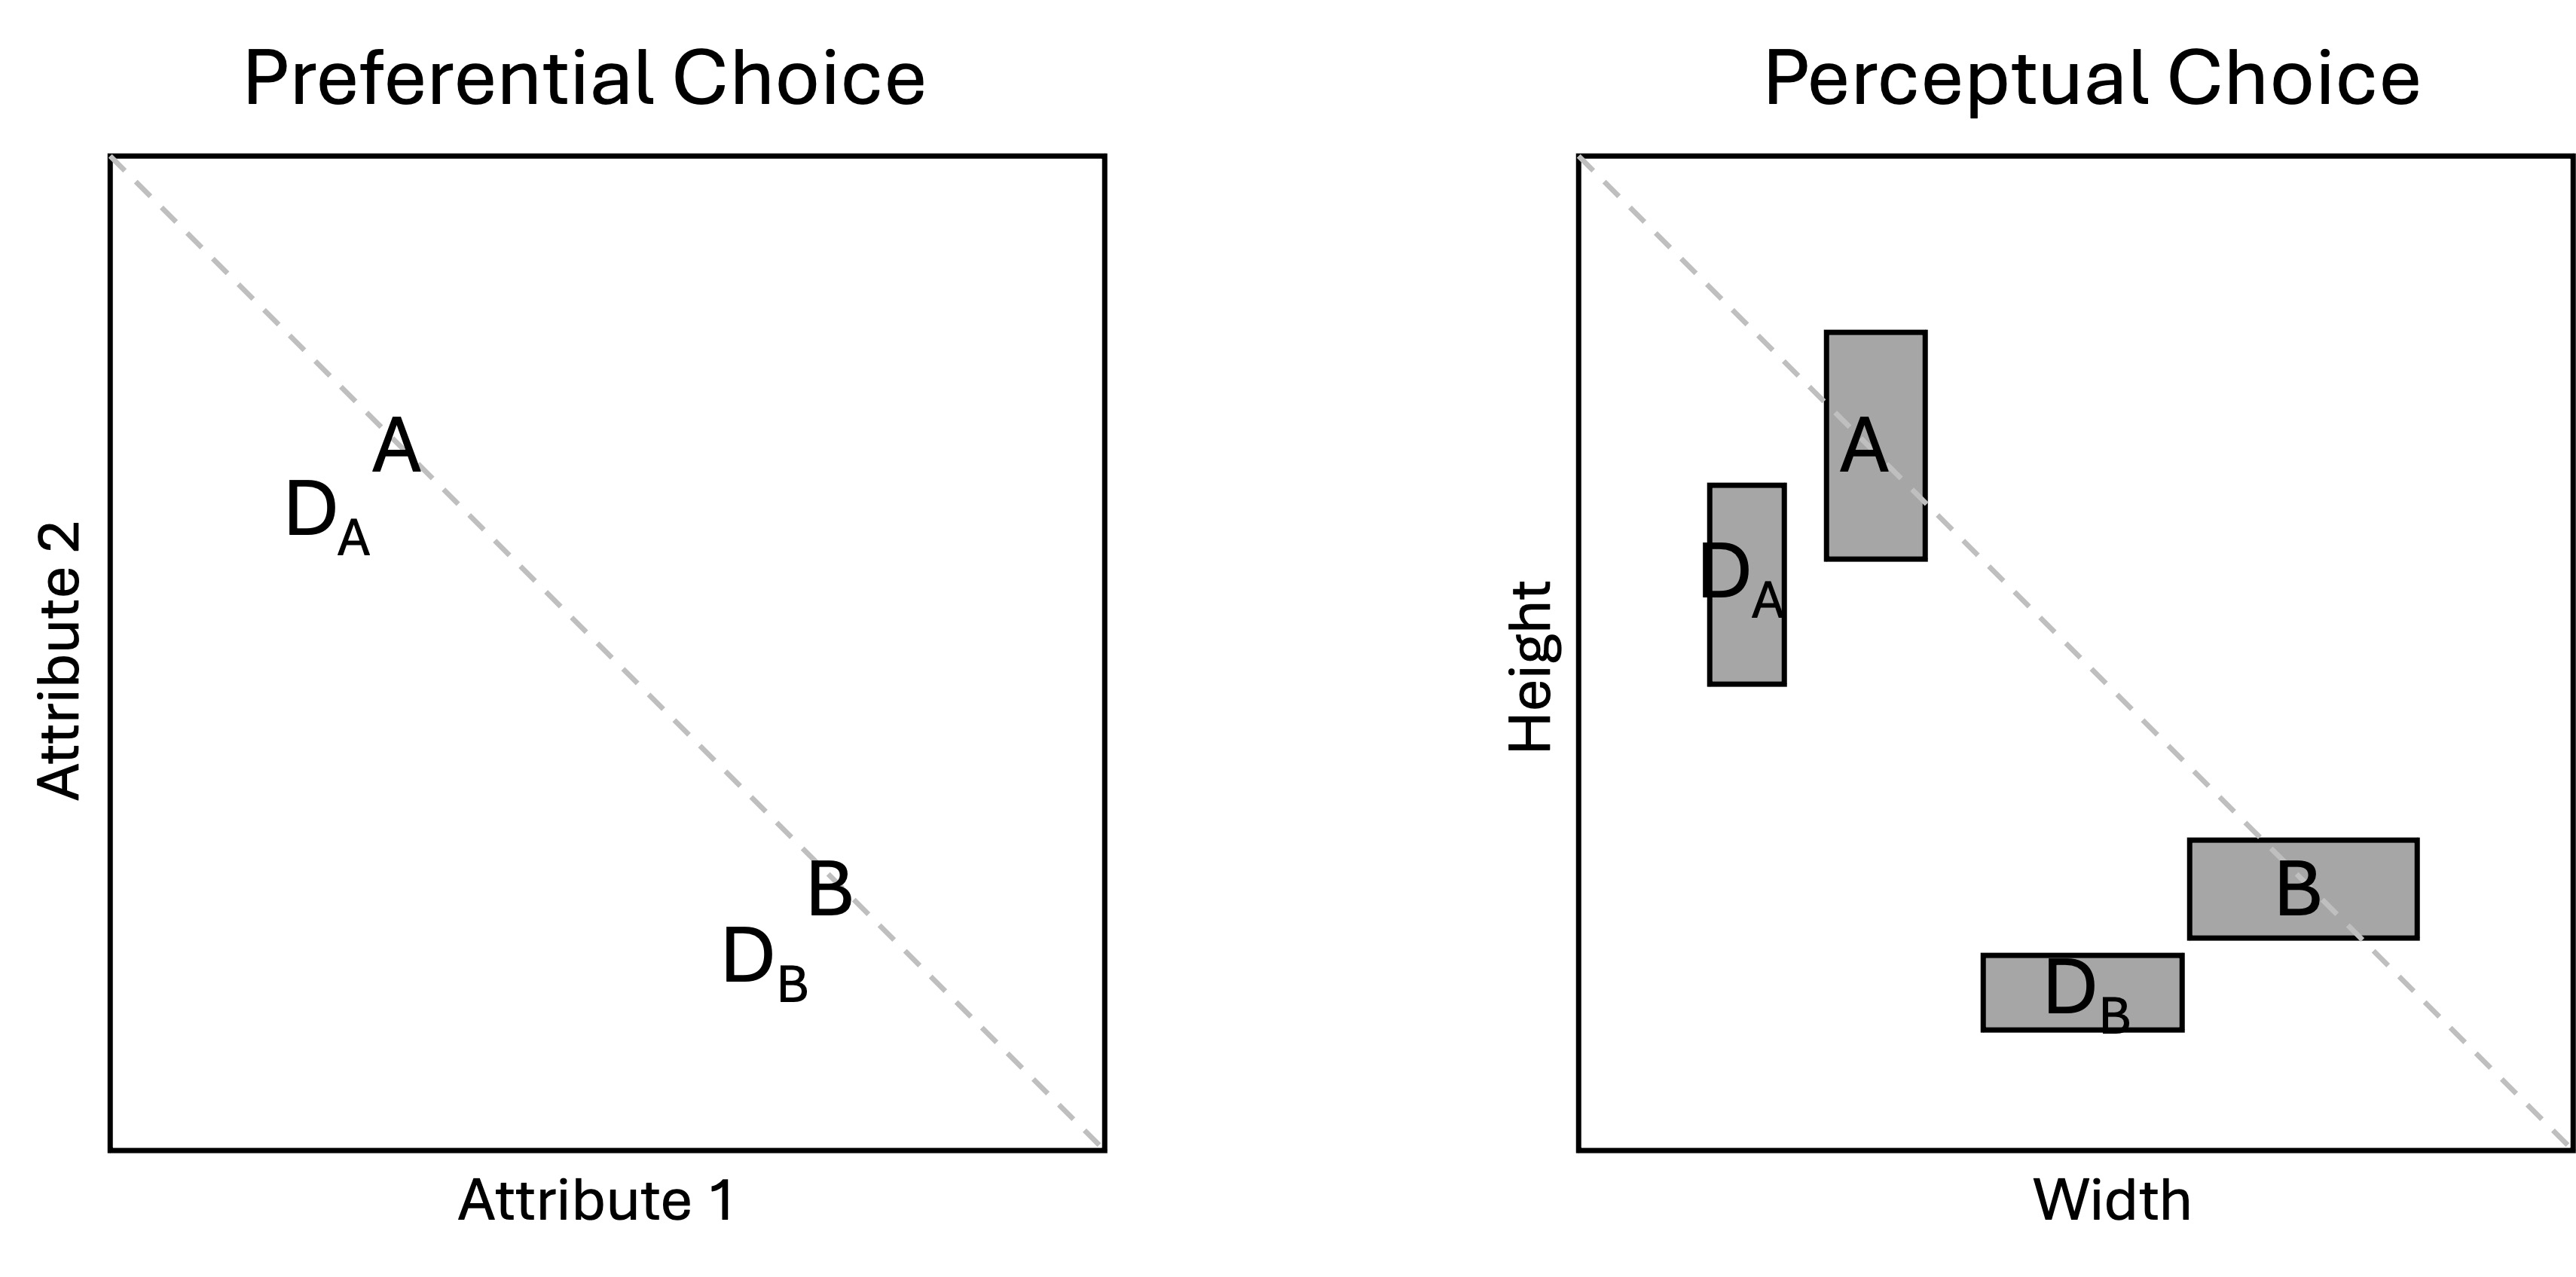
\includegraphics[width=\linewidth]{figures/pref_v_percep.jpg}
   \caption{A graphical depiction of choice options in the attraction/repulsion effect. Left panel: preferential choice. Right panel: perceptual choice.}
   \label{fig:fig_opts}
\end{figure}

According to IIA:

\begin{equation}
  \frac{P(A|[A,B,D_{A}])}{P(B|[A,B,D_{A}]}=\frac{P(A|[A,B,D_{B}])}{P(B|[A,B,D_{B}]}
  \label{eqn:iia}
\end{equation}

However, in the attraction effect, this equality is violated:

\begin{equation}
  \frac{P(A|[A,B,D_{A}])}{P(B|[A,B,D_{A}]}>\frac{P(A|[A,B,D_{B}])}{P(B|[A,B,D_{B}]}
  \label{eqn:iia_att}
\end{equation}

Thus, IIA is violated by the attraction effect\footnote{IIA is also violated by the repulsion effect, with the $>$ in Equation~\ref{eqn:iia_att} becoming a $<$.}.

In the context effects literature, it is common to refer to the similar, dominated option as the \textit{decoy}, the similar dominating option as the \textit{target}, and the dissimilar dominating option as the \textit{competitor}. For example, in the choice set $[A,B,D_{A}]$, $A$ is the target, $B$ is the competitor, and $D_{A}$ is the decoy. I adopt this terminology through this dissertation. 

The decoy is dominated by the target, so no rational agent should intentionally select it over the target, assuming they correctly perceive this dominance relationship.

The attraction effect was first demonstrated by \textcite{huberAddingAsymmetricallyDominated1982d} \footnote{These authors referred to this finding as the asymmetric dominance effect. To stay consistent with contemporary research, I use the term attraction effect throughout this dissertation.}, who tested participants with duples and triples of choice options, using products such as cars, beers, and TV sets. The authors showed that the introduction of an asymmetrically dominated decoy tended to increase the choice share of a similar, target option. Such a result violates IIA but also a principle known as regularity, which states that the introduction of another option to a choice set cannot increase the probability of choosing any given option:

\begin{equation}
  P(A|[A,B])\geq P(A|[A,B,D_{A}])
  \label{eqn:reg_att}
\end{equation}

\textcite{huberAddingAsymmetricallyDominated1982d}'s finding that $P(A|[A,B])\leq P(A|A,B,D_{A})$ therefore violates regularity. \textcite{huber1983market} replicated these results and also showed that if the decoy has a relatively high value, it can actually take choice shares away from the target. This result suggests that the relative positioning of the decoy to the target can greatly affect patterns of choice, a finding explored by numerous other researchers which has strong theoretical consequences.

Numerous researchers have since demonstrated the attraction effect in preferential choice, including in real-world scenarios. \textcite{doyleRobustnessAsymmetricallyDominated1999} found an attraction effect in real world supermarket choices by adding a decoy option to an existing product set, where the decoy option was the same brand and price as the target, but of a lower volume. \textcite{van2021attract} showed that the attraction effect can be used to induce people to choose healthier food items. \textcite{slaughterDecoyEffectsAttributelevel1999b} showed that the attraction effect can be found even without the explicit attribute descriptions commonly used in laboratory experiments, when participants must infer option attributes. Researchers have demonstrated other context effects, such as the similarity effect, where a similar but equally valuable decoy \textit{decreases} the choice share of a target option \parencite{tverskyEliminationAspectsTheory1972}, and the compromise effect, where an intermediate option decreases the choice share of two relatively extreme options \parencite{simonsonChoiceBasedReasons1989b}. 

Context effects have strong theoretical implications. Traditional models of choice, as used in economics and marketing research \parencite{mcfadden2001economic}, treat the \textit{utility}, or value, of each option as a random variable whose parameters are estimated from choice data. According to these models, on each trial of a choice experiment the participant samples values from these distributions and deterministically chooses the option with the highest sampled value. These models are known as \textit{Random Utility Models} (RUMs). When utilities are assumed to follow a Type 1 Generalized Extreme Value distribution, the logit or softmax model is used \parencite{gensch1979multinomial}. As will be the focus of much of this dissertation, the probit model assumes Gaussian distributed utilities \parencite{bolduc1999practical}. Often (though not necessarily) RUMs assume IIA (c.f,. \textcite{paetzUtilityIndependenceIIA2018}), though this assumption can be relaxed by estimating choice set or alternative specific coefficients \parencite{rooderkerk2011incorporating} or allowing correlations between options and/or attributes \parencite{haaijer1998utility}. If IIA is assumed, RUMs are unable to account for context effects \parencite{berkowitschRigorouslyTestingMultialternative2014b}. 

In cognitive psychology, researchers have developed process models that attempt to explain the mental processes that lead to context effects \parencite{trueblood2014multiattribute,roeMultialternativeDecisionField2001a,busemeyerCognitiveNeuralBases2019, usherLossAversionInhibition2004a,bhatiaAssociationsAccumulationPreference2013b,noguchiMultialternativeDecisionSampling2018a,wollschlager2NaryChoiceTree2012a,bergnerVAMPVotingAgent2019b,tverskyEliminationAspectsTheory1972,tversky1993context}. These models differ, to varying degrees, in their explanations for the attraction effect. Many, however, rely on comparisons between the target and the similar, but inferior, decoy, which boost an internal  preference state for the target. \textcite{roeMultialternativeDecisionField2001a}'s Multialternative Decision Field Theory (MDFT) model proposes that the similarity between target and decoy causes frequent target-decoy comparisons, and through lateral inhibition, the negative valence for the decoy causes a boost to the preference state of the target at the expense of the competitor. \textcite{trueblood2014multiattribute}'s Multiattribute Linear Ballistic Accumulator (MLBA) model proposes that pairwise attention weights, which are a function of the similarity between options, increase the importance of target-decoy comparisons and thus boost preference for the target. 

This dissertation does not explore the predictive success of these models, nor does it incorporate model fitting to compare these models. Indeed, other researchers have performed such analyses \parencite{turnerCompetingTheoriesMultialternative2018a,cataldoModelingPreferenceReversals2021,evansResponsetimeDataProvide2019b,molloyWhatResponseTime2019a,berkowitschRigorouslyTestingMultialternative2014b,hotalingTheoreticalDevelopmentsDecision2010,cohen2017multi}, arriving at varying conclusions. Instead, I use behavioral experiments and statistical modeling to understand how context dependence arises in various domains.

The attraction effect is not solely limited to consumer choice. Researchers have demonstrated the attraction effect in risky choice \parencite{mohr2017attraction}, policy choice \parencite{herneDecoyAlternativesPolicy1997b}, intertemporal choice \parencite{mariniAttractionComesMany2020}, probability judgment \parencite{caiWhenAlternativeHypotheses2023}, medical decision-making \parencite{schwartz1999more}, episodic memory judgment \parencite{maylorSimilarityAttractionEffects2007b}, charitable donation \parencite{pittarello2020three},  inference \parencite{truebloodMultialternativeContextEffects2012}, job candidate selection \parencite{highhouseContextDependentSelectionEffects1996}, political choice \parencite{pan1995attractiovoting}, sports prediction \parencite{fang2024context}, and, as will be the focus of much of this dissertation, perceptual choice \parencite{evansImpactPresentationOrder2021,trueblood2013not, trueblood2015fragile, spektorRepulsionEffectPreferential2022,spektorWhenGoodLooks2018b,yearsleyContextEffectsSimilarity2022,turnerCompetingTheoriesMultialternative2018a,liaoInfluenceDistanceDecoy2021}. 

As I will discuss throughout this dissertation but particularly in Chapter 2, recent work has demonstrated inconsistency in context effects, particularly in perceptual choice. I use behavioral experiments and statistical in an attempt to reconcile these inconsistencies.

This dissertation is structured as follows. In Chapter 2, I develop and test a statistical model of perceptual variability when applied to context effects. In Experiment 1, I first show that the types of stimuli used in perceptual choice context effects experiments are easily confusable and vary systematically with theoretically relevant properties of the stimuli. In Experiment 2, I use the results of a high-powered psychophysics experiment to show that the repulsion effect, but not the attraction effect, is naturally predicted by this statistical model. In Chapter 3, I further test the statistical model by applying it to best-worst choice. In Chapter 4, I generalize the paradigm and model to preferential choice. Finally, in Chapter 5, I use a perceptual choice experiment to show that stimulus comparability affects choice, even when the decoy is equally similar to both focal options. In Chapter 6, I summarize the findings of the dissertation, their implications, and discuss future directions for research in this domain. 
